%Vorlage Uni, made by Oliver Wisler 25.20.2011

%set document language to german, standard font size and document size
\documentclass[ngerman, 12pt, pdftex]{scrartcl}[2006/07/30]

%encoding and input
\usepackage[ngerman]{babel} %spell correction
\usepackage[utf8]{inputenc} 
\usepackage[T1]{fontenc}

%bugfixes
\usepackage{fixltx2e} 

%Font Symbols and Colors
\usepackage{textcomp} %more symbols
\usepackage{xcolor}

%Math
\usepackage{amsmath}
\usepackage{mathtools} %extends amsmath

%Programming
\usepackage{listingsutf8} %in utf8d
\lstset{language=Java,captionpos=b,tabsize=3,frame=lines,keywordstyle=\color{blue},commentstyle=\color{teal},stringstyle=\color{red},numbers=left,numberstyle=\tiny,numbersep=5pt,breaklines=true,showstringspaces=false,basicstyle=\footnotesize,emph={label},upquote=true} %Syntax highlighting

%Verbatim extension (with line numbers and tab-expansion)
\usepackage{moreverb} 

%graphics
\usepackage{graphicx}

%Headers and Footer
\usepackage{fancyhdr}

%title
\title{CS261 Webprojekt}
\author{Frank Müller, Oliver Wisler}

\begin{document}
%declare  Header
\pagestyle{fancy}
\fancyhf{} 
\fancyhead[L]{cs261 Webprojekt} %left header
\fancyhead[C]{Meilensteine} %centered header
\fancyhead[R]{Frank Müller, Oliver Wisler}  % right header
\renewcommand{\headrulewidth}{0.1pt} 	%upper separating line
\fancyfoot[C]{\thepage} 				%centered footer, line number
%\renewcommand{\footrulewidth}{0.1pt} 	%lower separating line




%%%%%CONTENT%%%%%
%you might want to enable come features:
%\maketitle
\tableofcontents
\newpage


\section{Meileinstein 1}
\subsection{Navigation}
Die Navigation soll möglichst einfach sein. Es gibt sehr wenige Unterseiten, so dass die gesamte Funktionalität in innerhalb weniger Seiten zur Verfügung steht. 
\begin{figure}[h!]
\center
	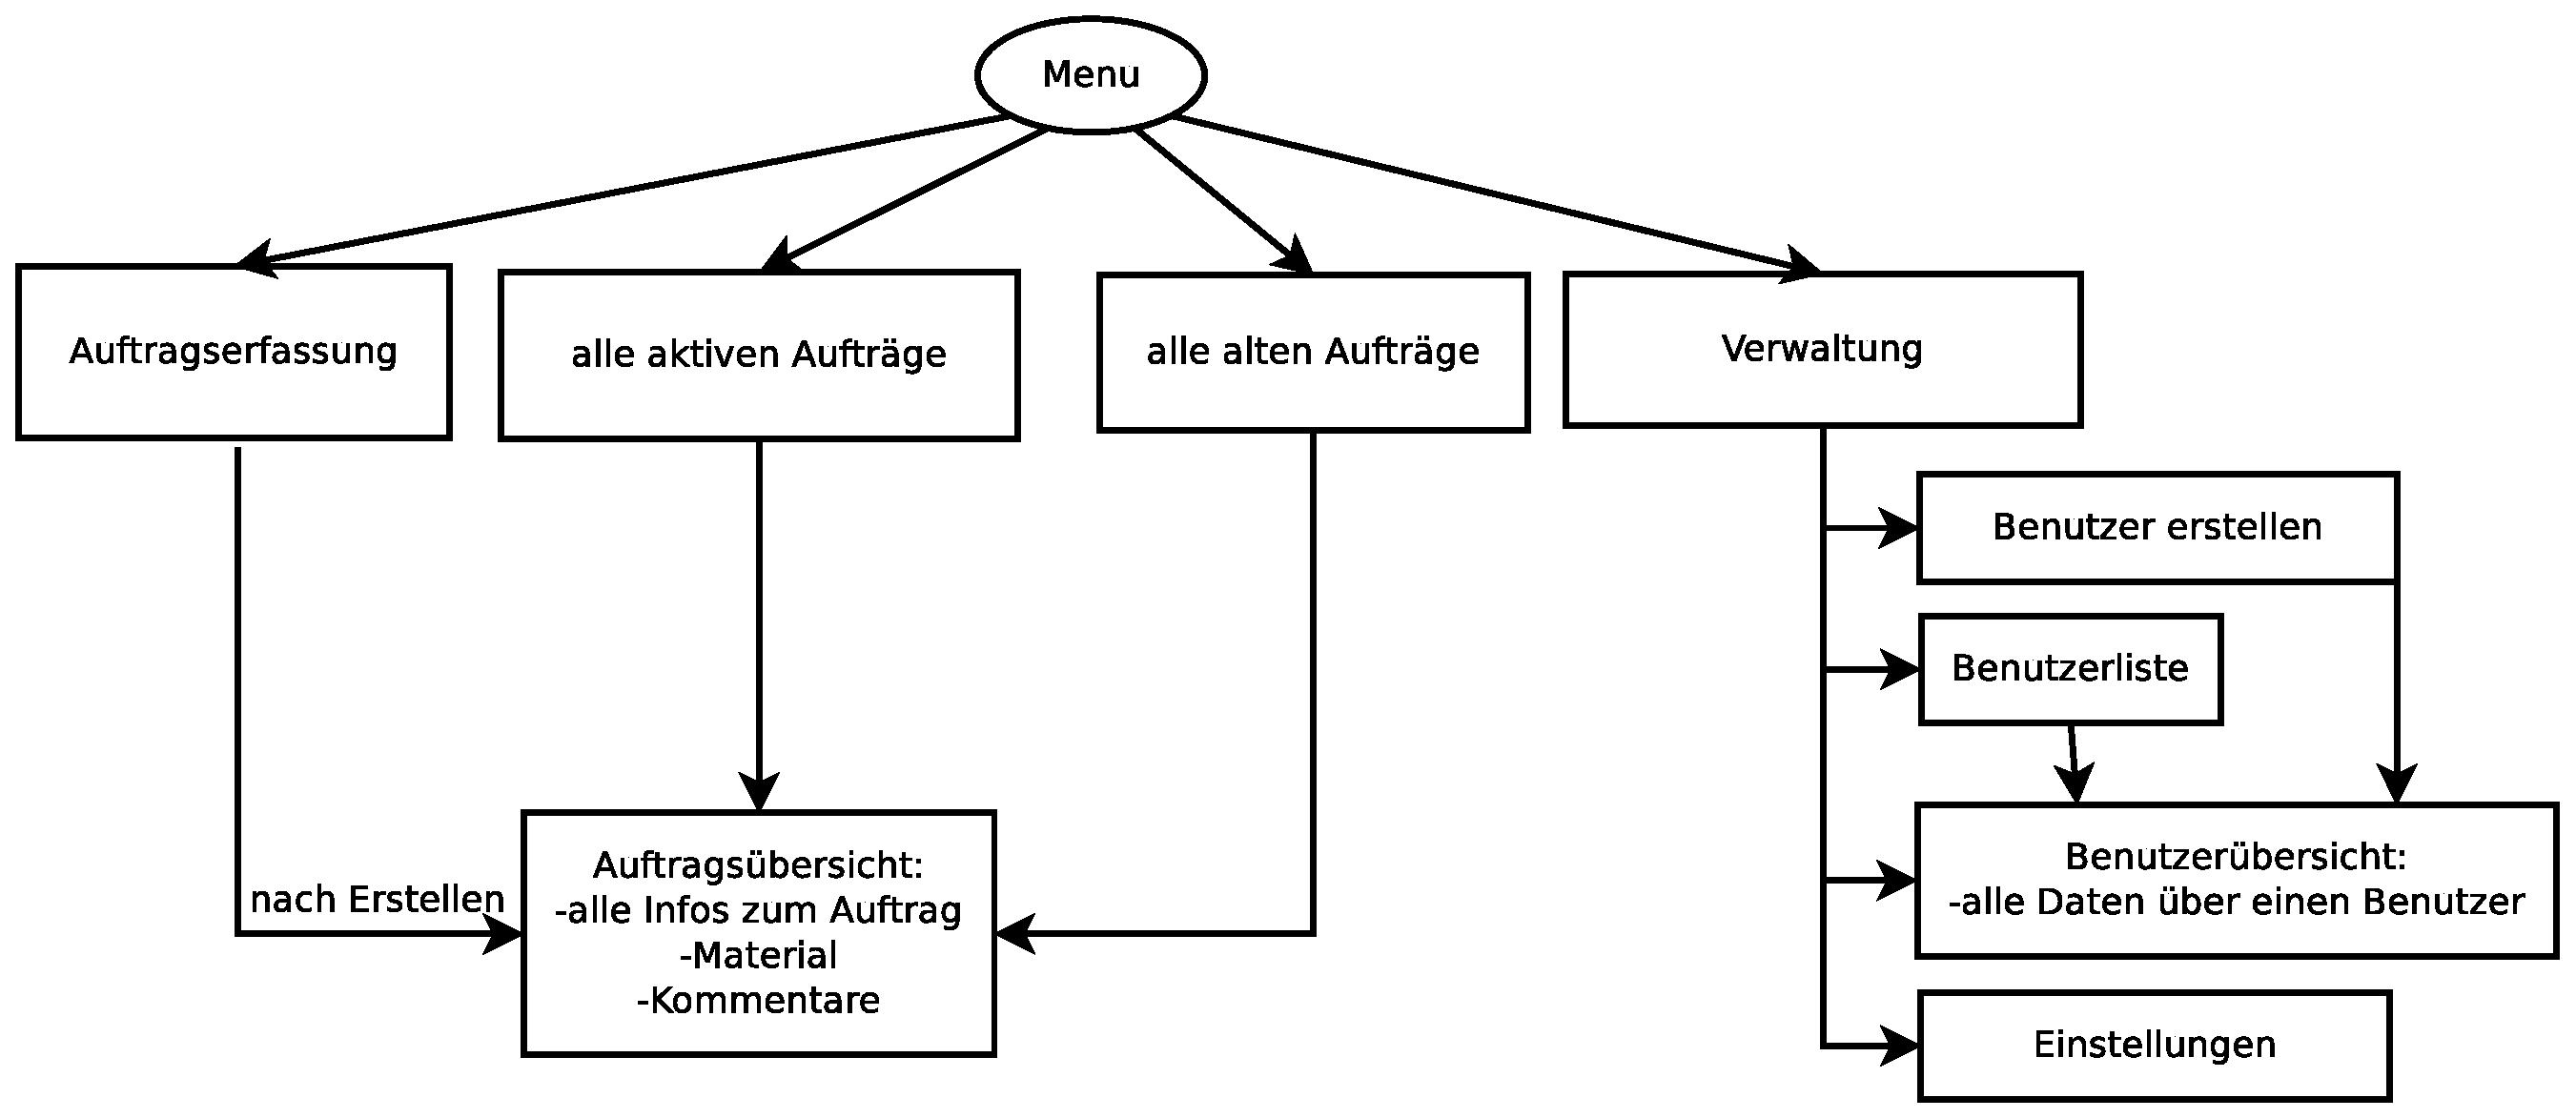
\includegraphics[scale=0.35]{./navigation.eps}
	
\end{figure}


\subsection{Design}
Unsere Seite soll schlicht und nicht überladen sein. Ziel ist es, eine möglichst einfache und simple Oberfläche zu haben. Der Benutzer soll effizient arbeiten können, ohne vom Design abgelenkt oder darin behindert zu werden.
Wichtige Informationen und Hinweise werden farblich hervorgehoben.

\begin{figure}[p]
\centering
	\begin{minipage}{0.4\textwidth}
		\centering
		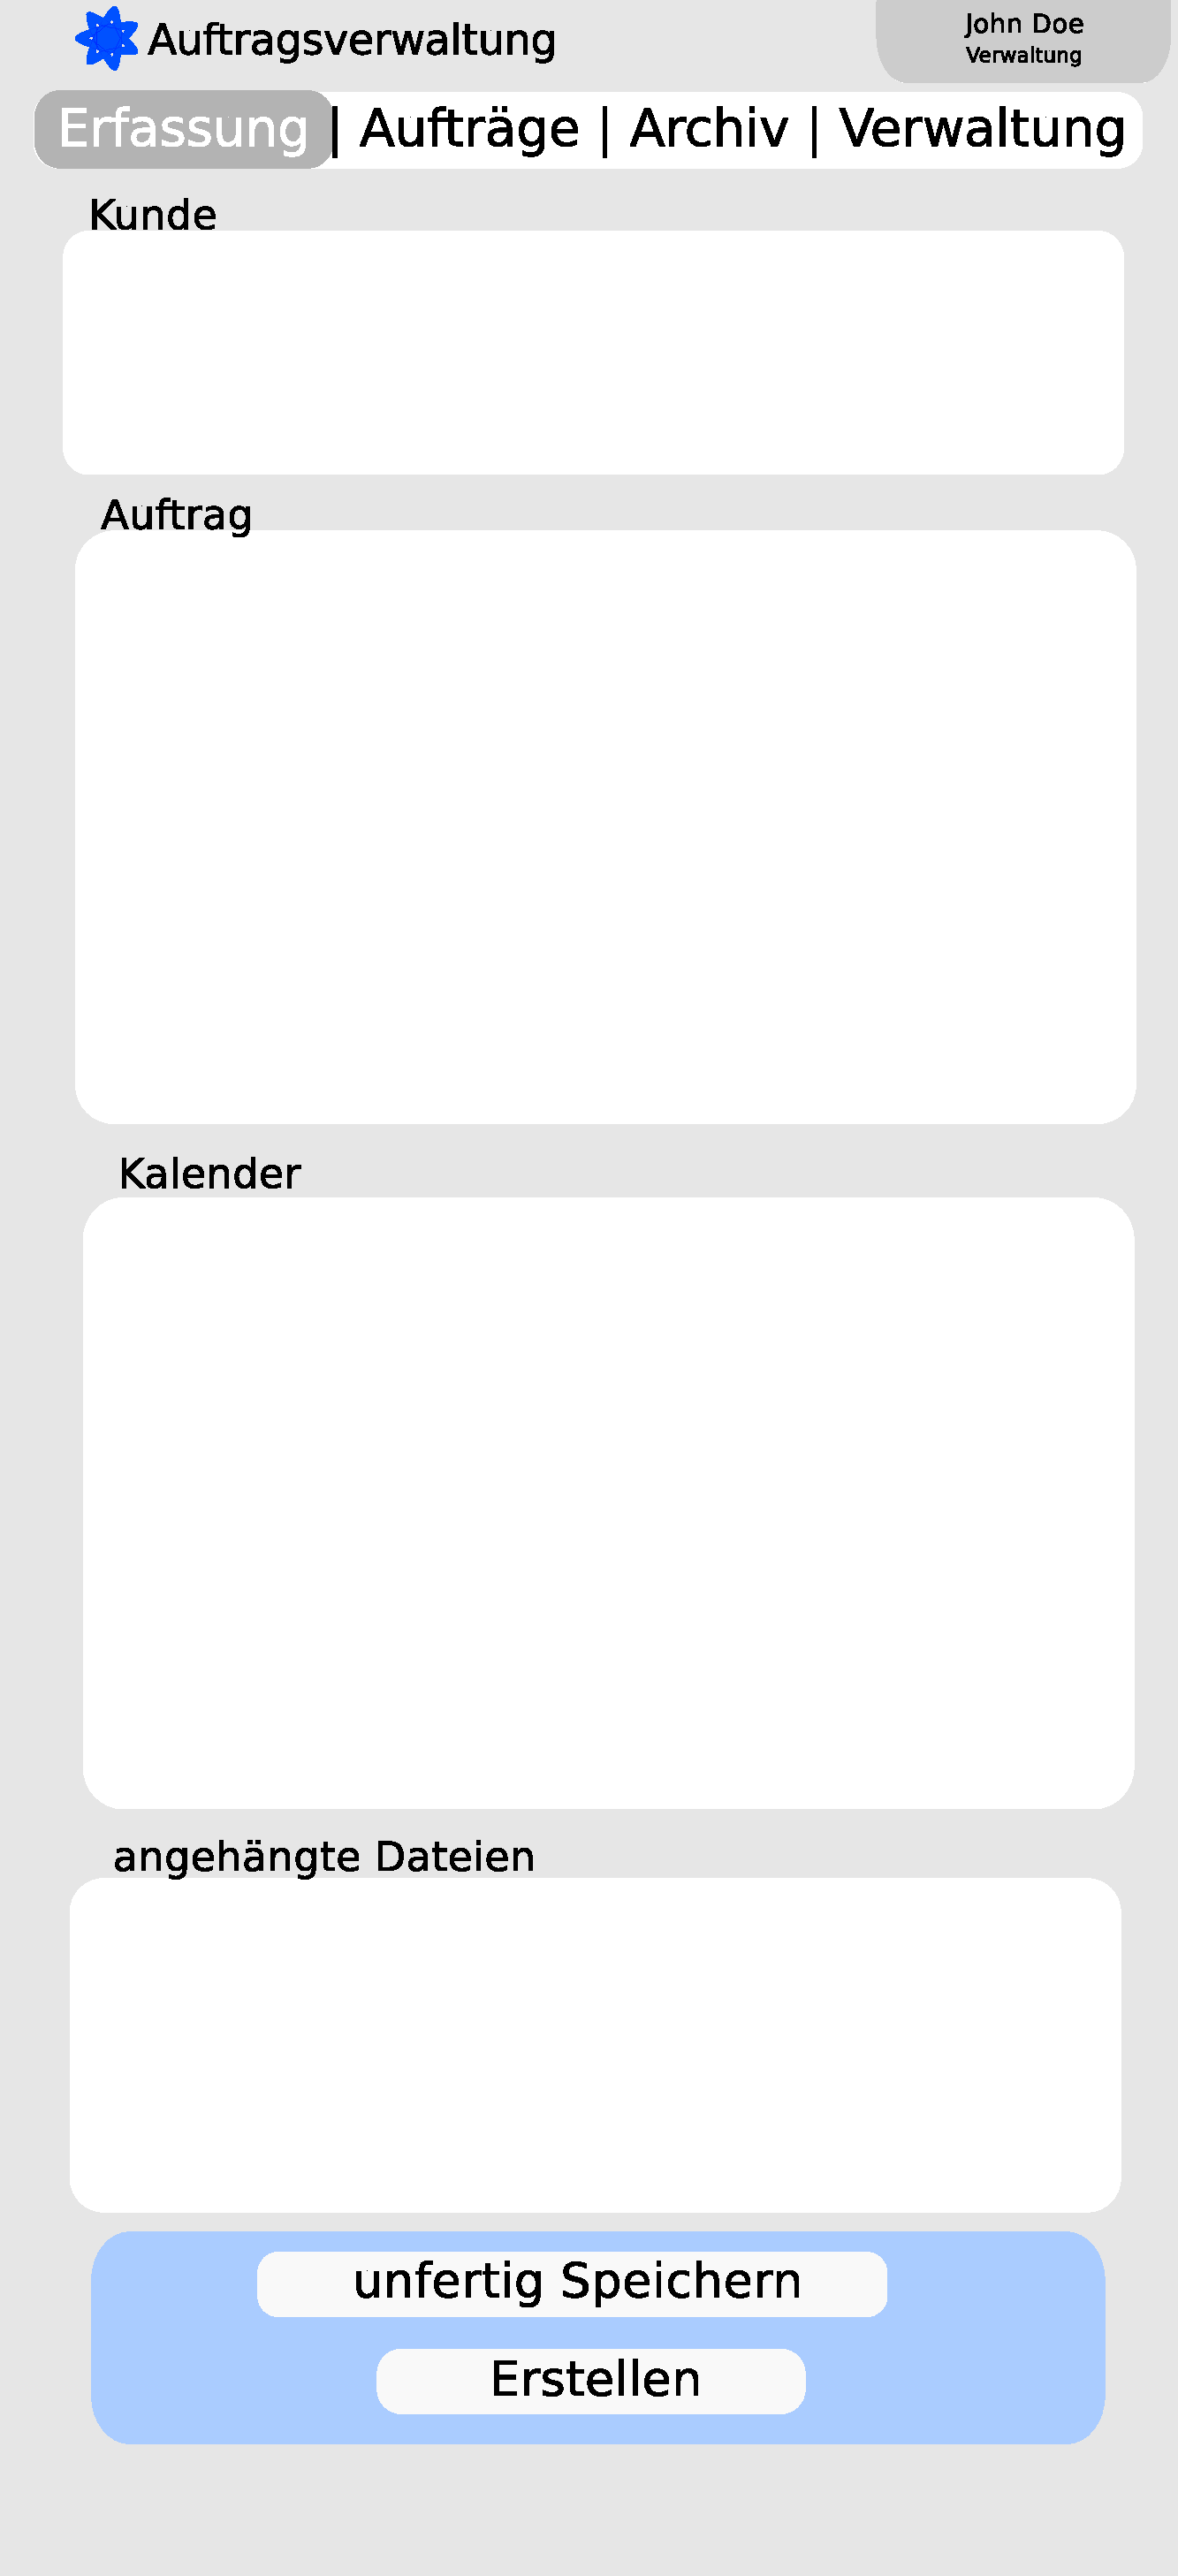
\includegraphics[scale=0.3]{./design/create_order.pdf}
		\caption{Erstellen eines Auftrages}
 	\end{minipage}\hfill
    \begin{minipage}{0.4\textwidth}
   		\centering
   		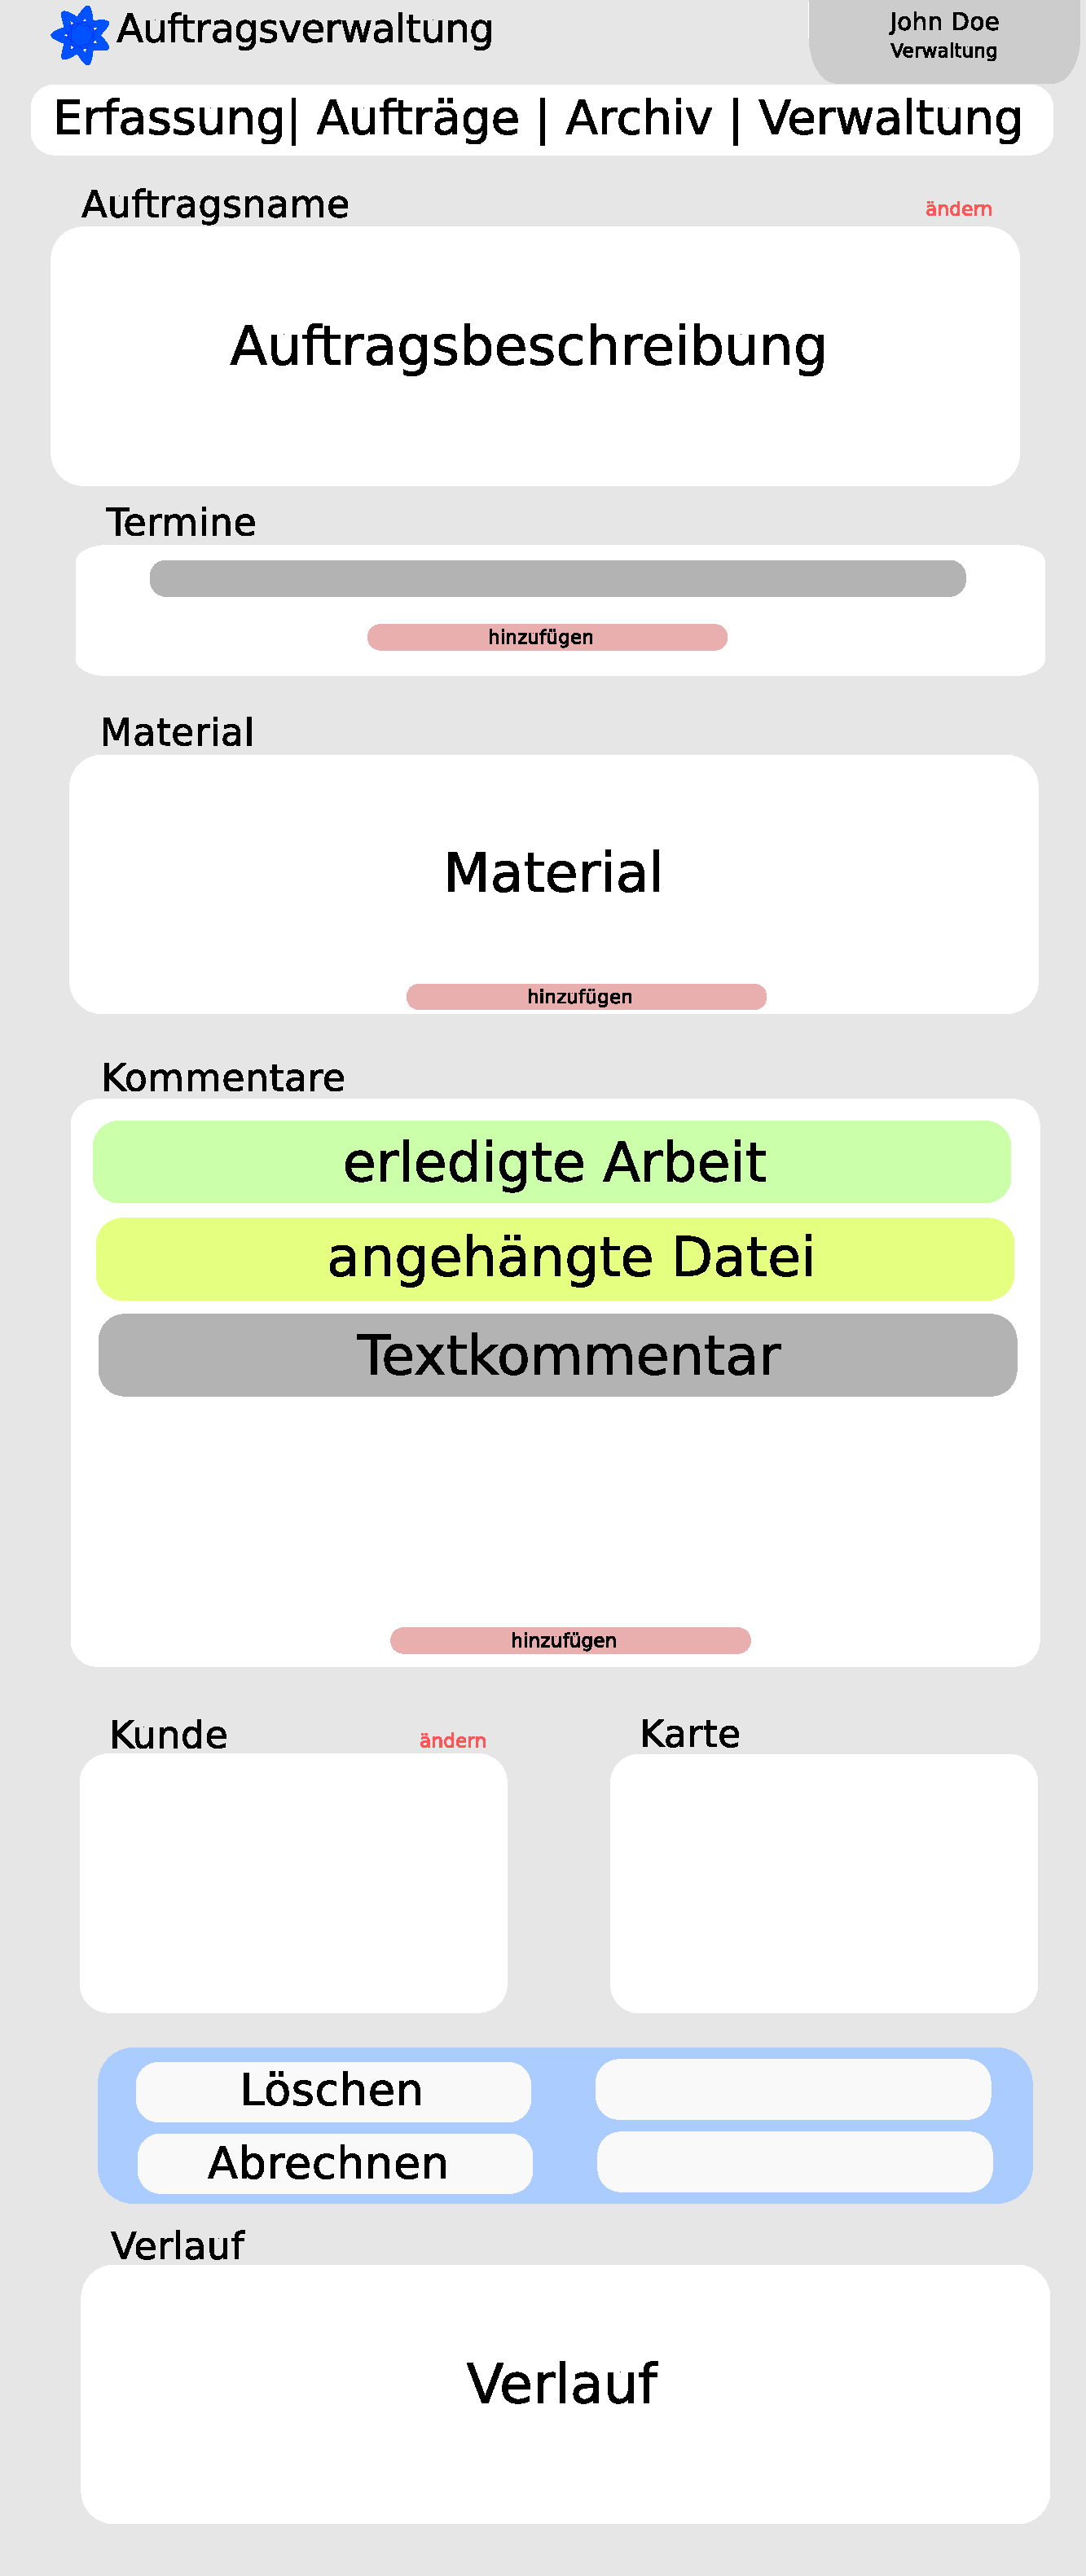
\includegraphics[scale=0.3]{./design/change_order.pdf}
		\caption{Auftragsübersicht}
	\end{minipage} 
	
\end{figure}
\begin{figure}[p]
\centering
	\begin{minipage}{0.4\textwidth}
		\centering
		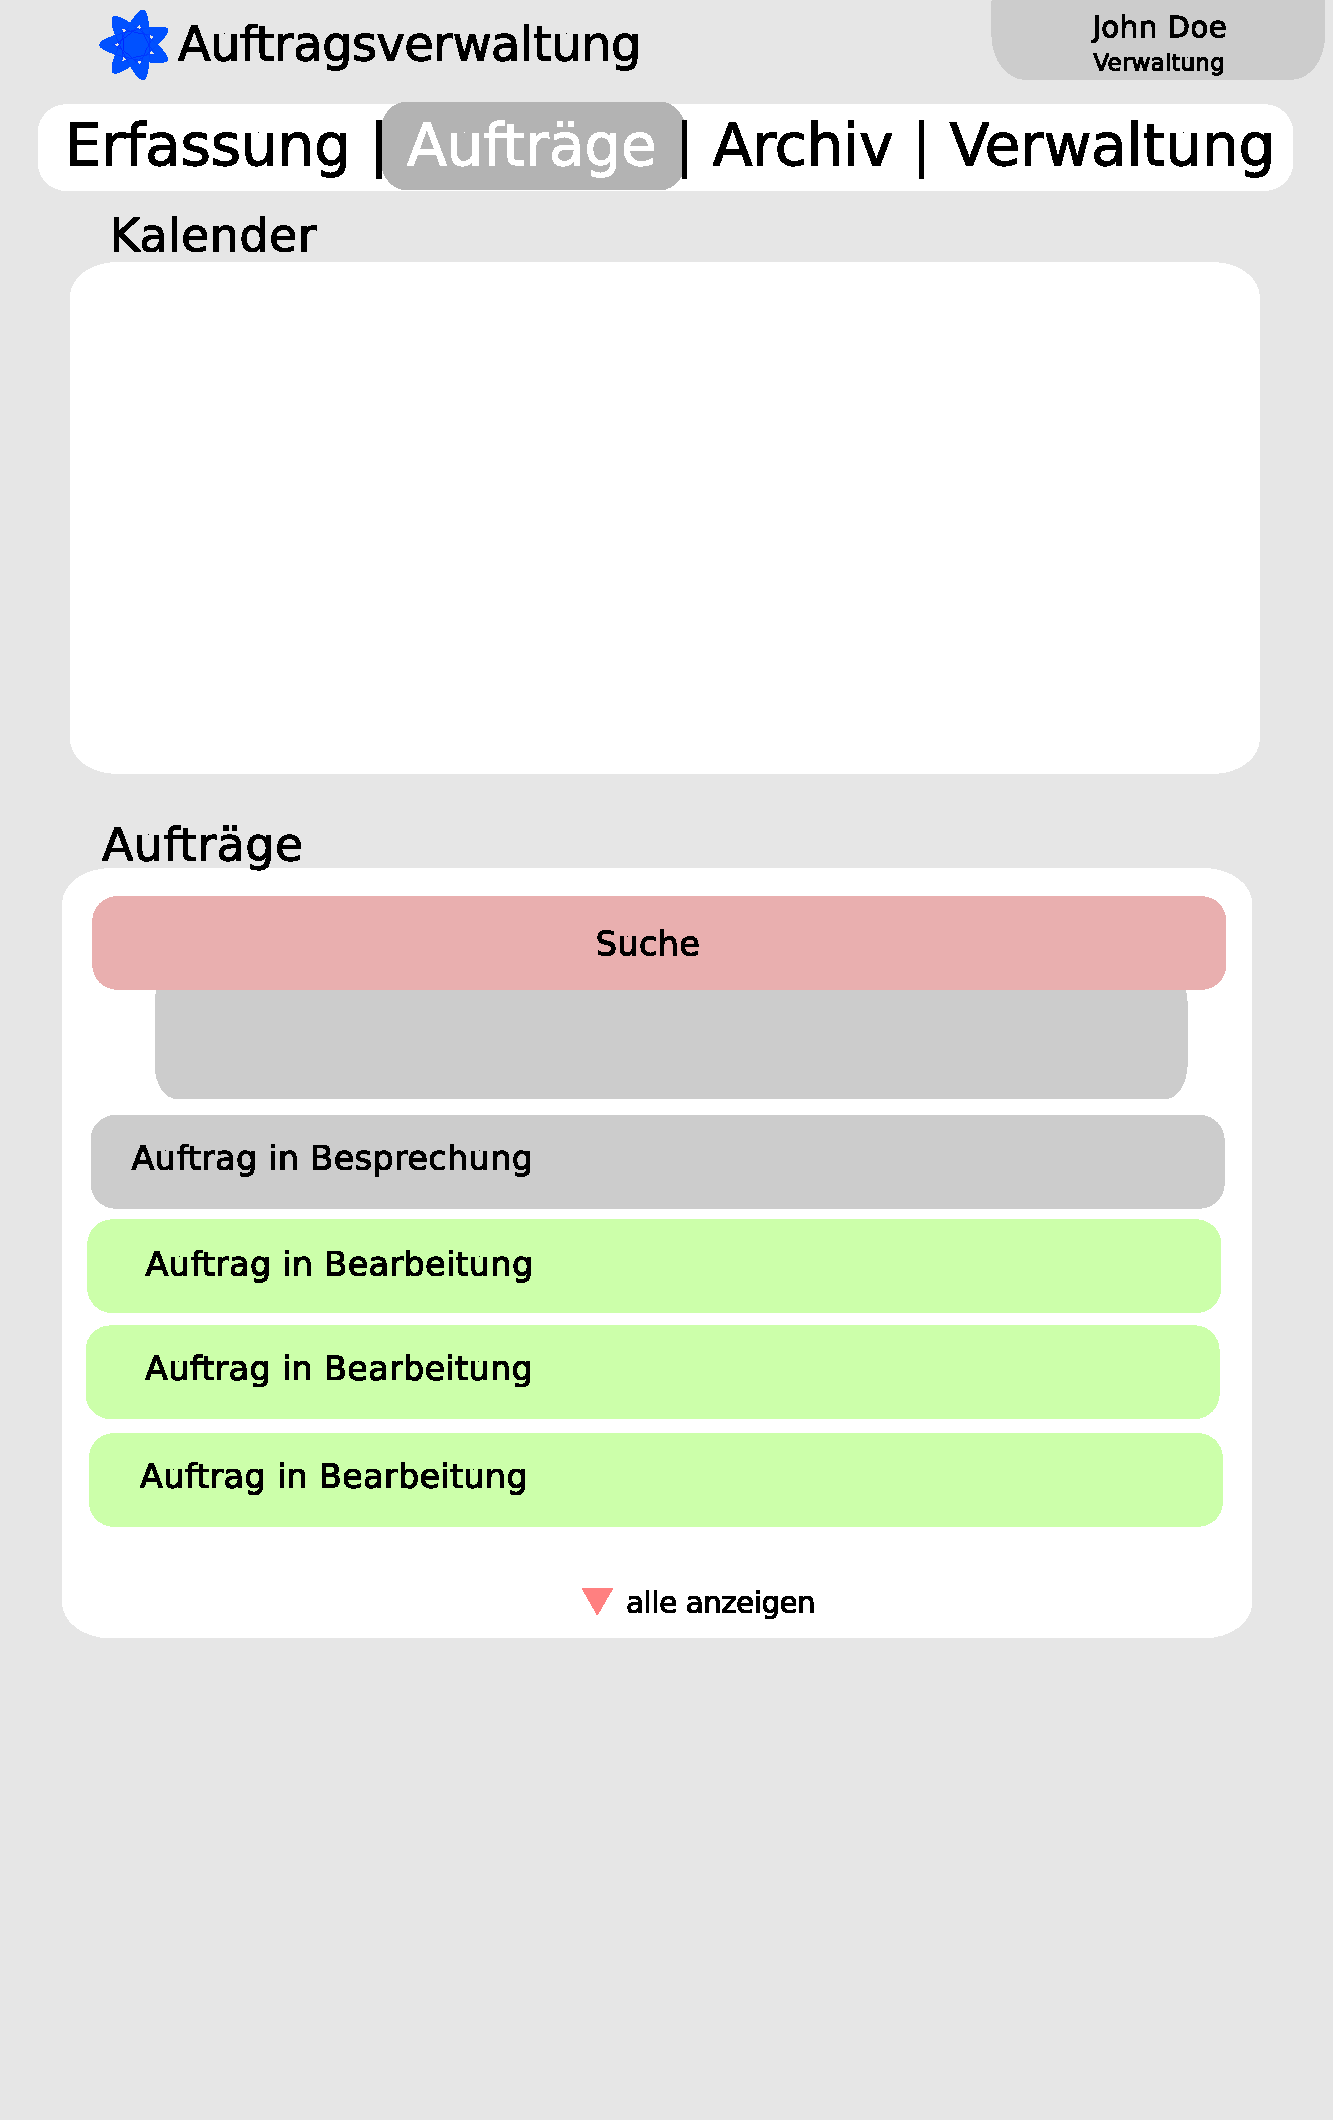
\includegraphics[scale=0.3]{./design/overview_order.pdf}
		\caption{Alle pendenten Aufträge}
 	\end{minipage}\hfill
    \begin{minipage}{0.4\textwidth}
   		\centering
   		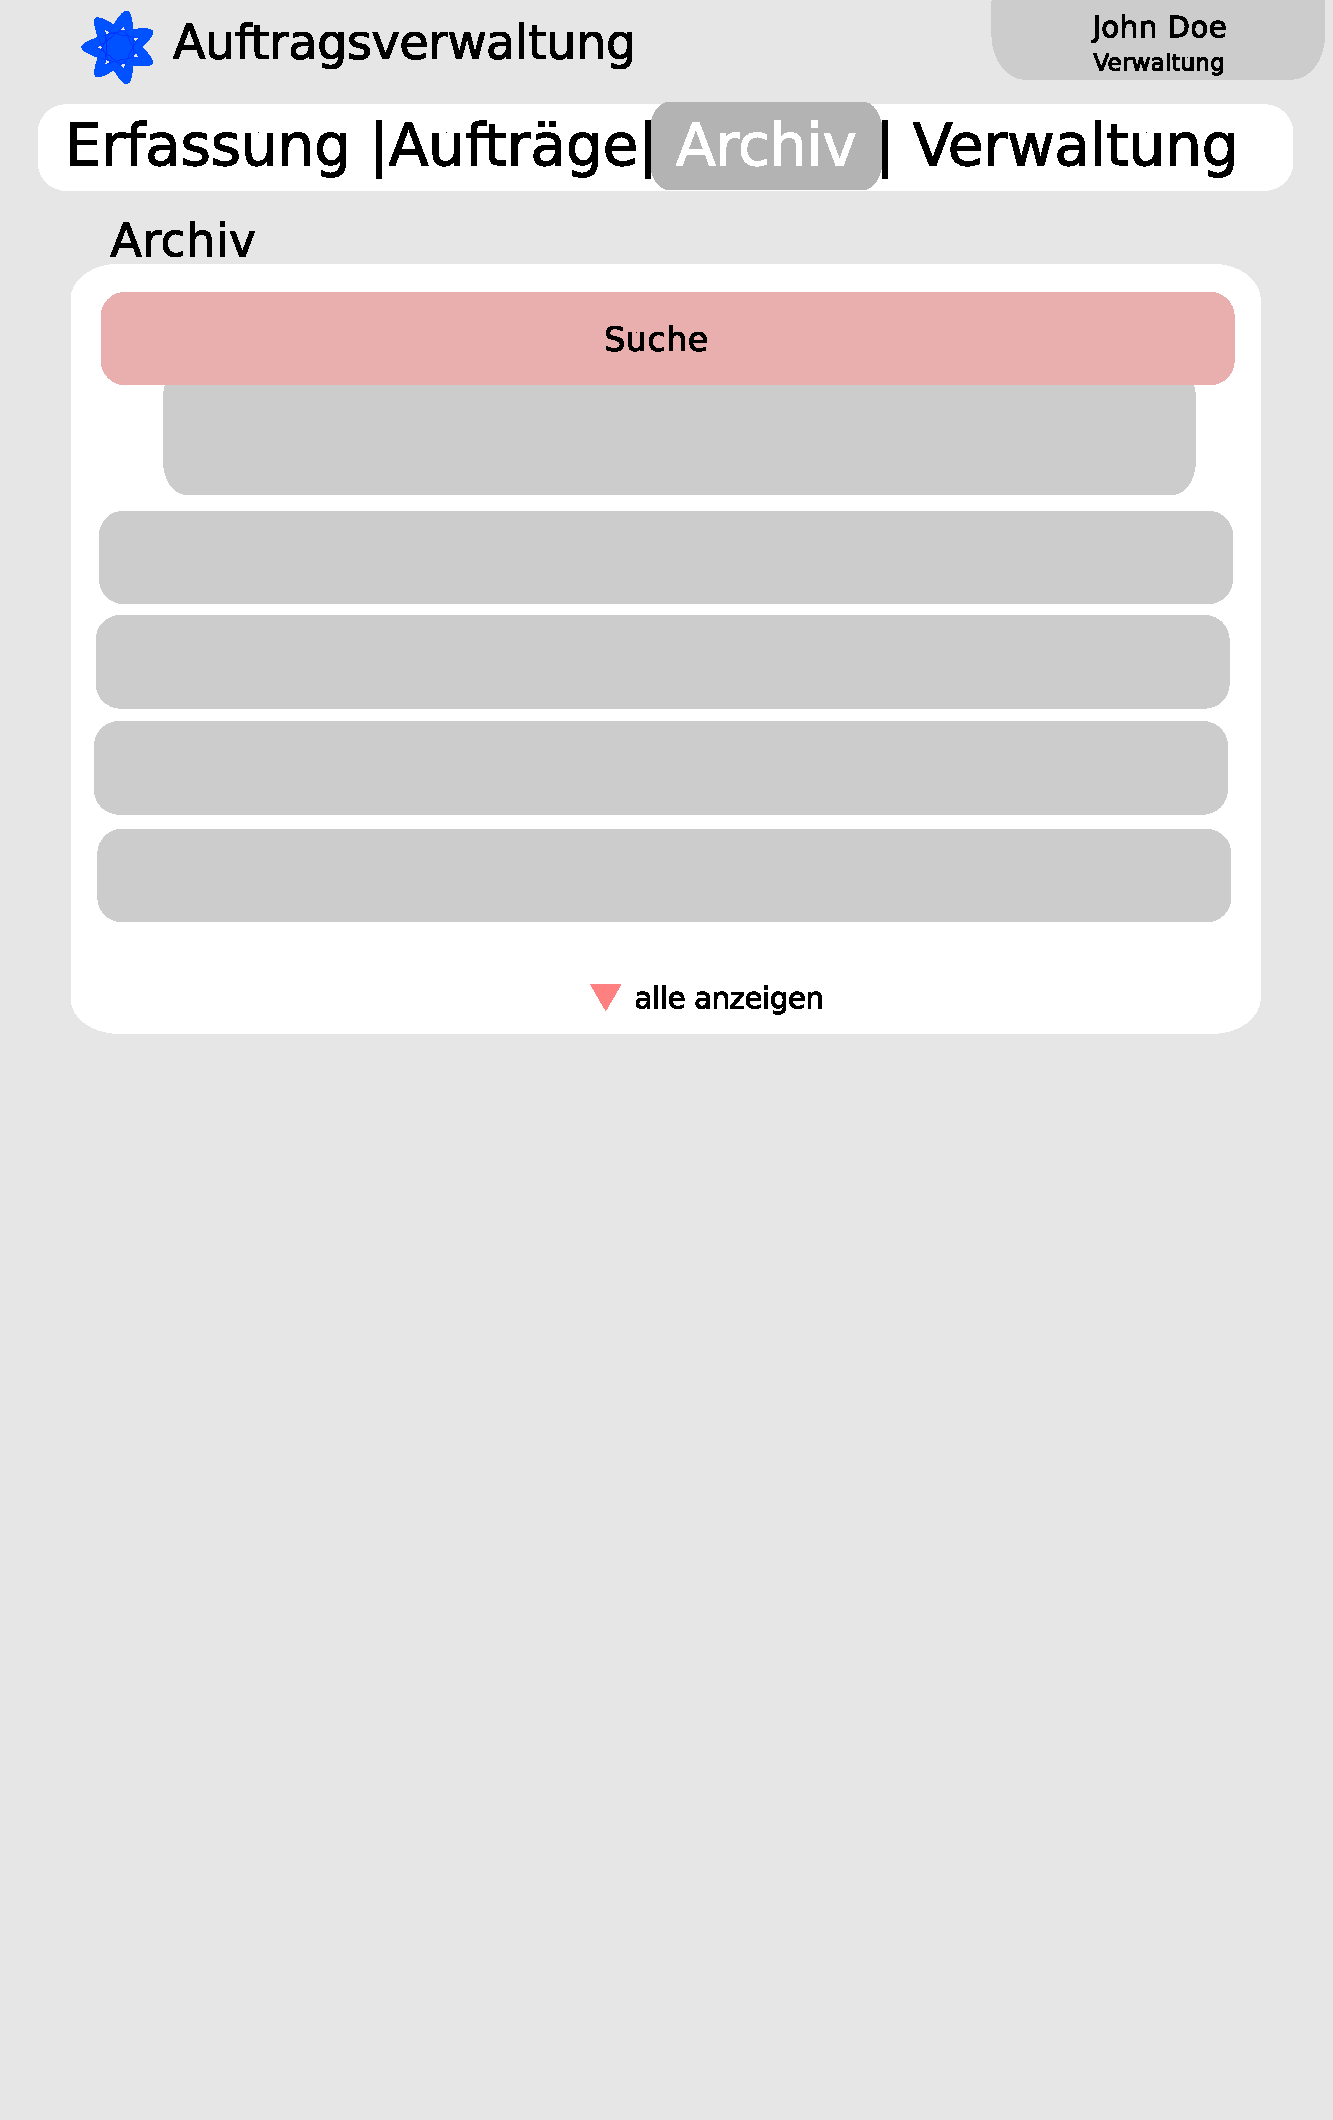
\includegraphics[scale=0.3]{./design/archive_order.pdf}
		\caption{Archiv aller abgeschlossenen Aufträge}
	\end{minipage} 
	
\end{figure}

\subsection{Datenbank}
Wir werden eine MySQL Datenbank verwenden. Für eine genauere Ansicht finden Sie die Dokumente unter 
 \verb+./db_prefs/*.pdf+.


\begin{figure}[p]
	\centering
	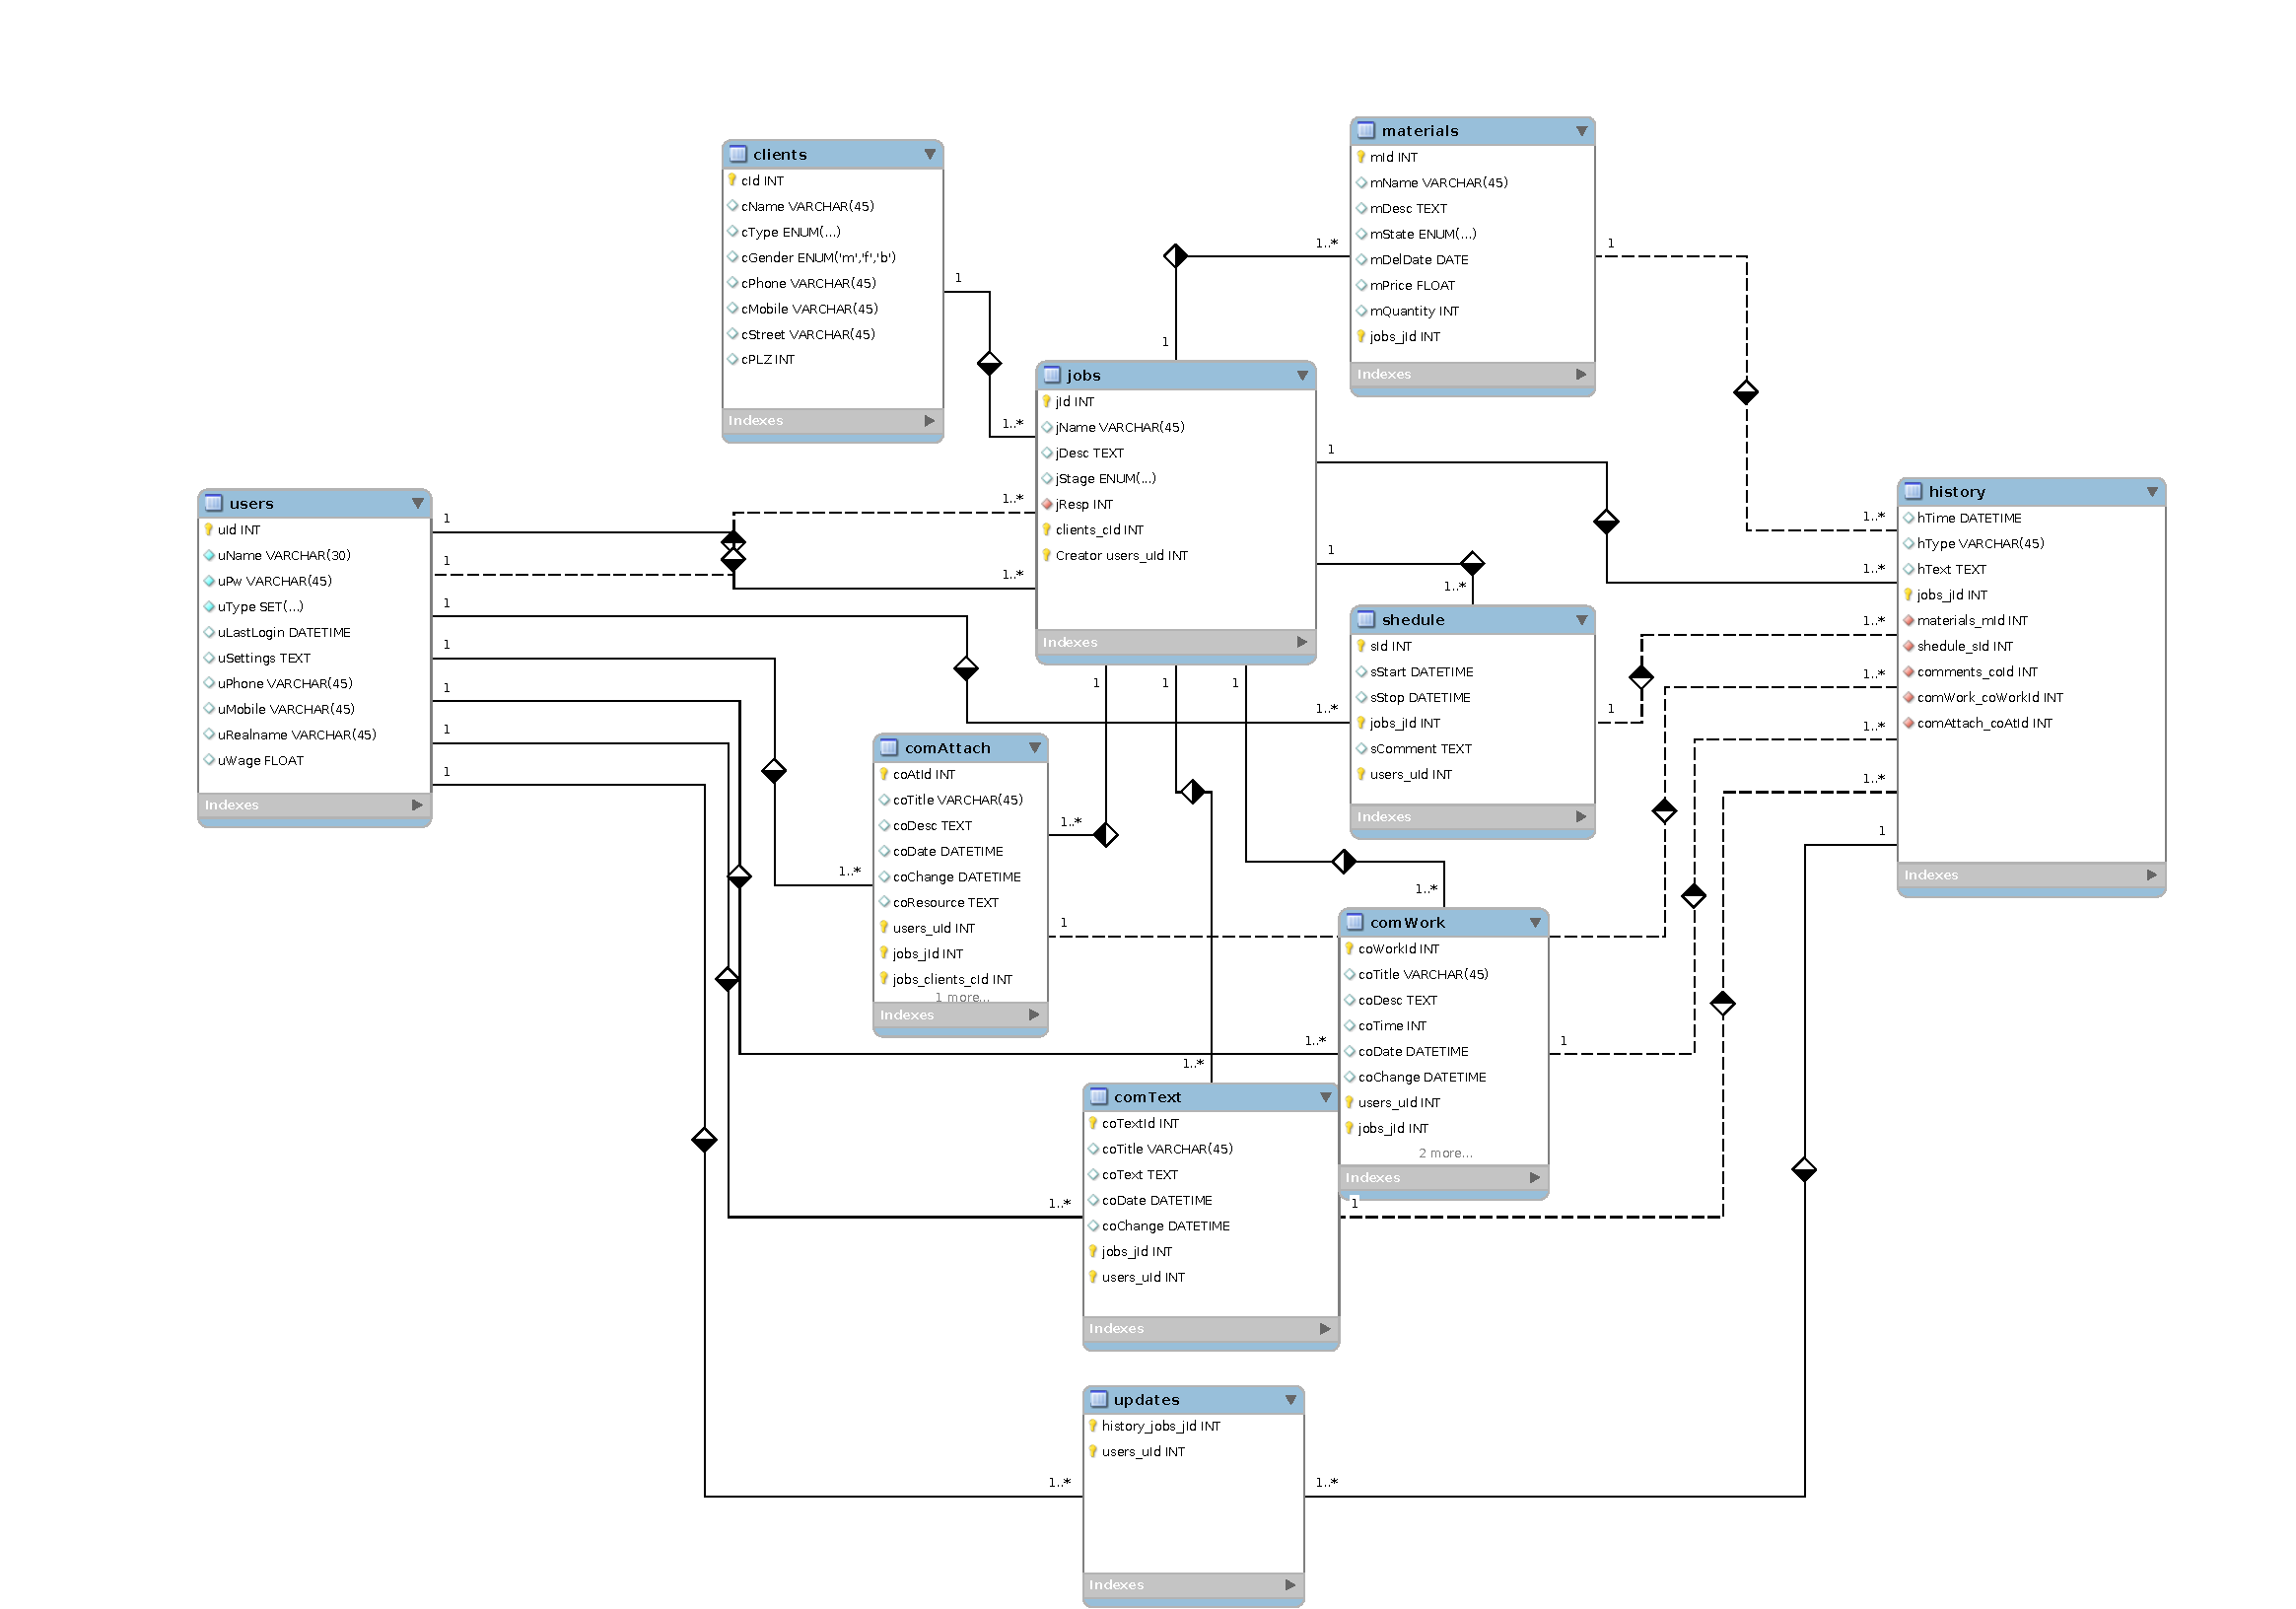
\includegraphics[scale=0.4]{./db_pdfs/everything.pdf}
	\caption{Das gesamte Datebankschema}
\end{figure}

\begin{figure}[p]
	\centering
	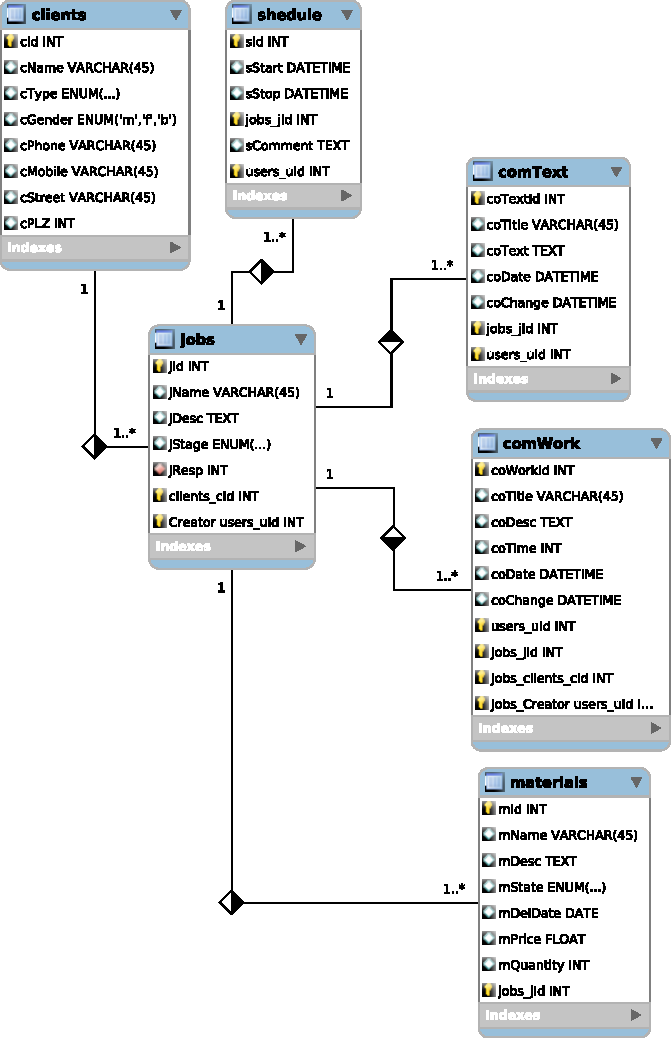
\includegraphics[scale=1]{./db_pdfs/jobs.pdf}
	\caption{Alle Tabellen in denen Informationen betreffend eines Auftrages sind.}
\end{figure}

\begin{figure}[hbt]
	\centering
	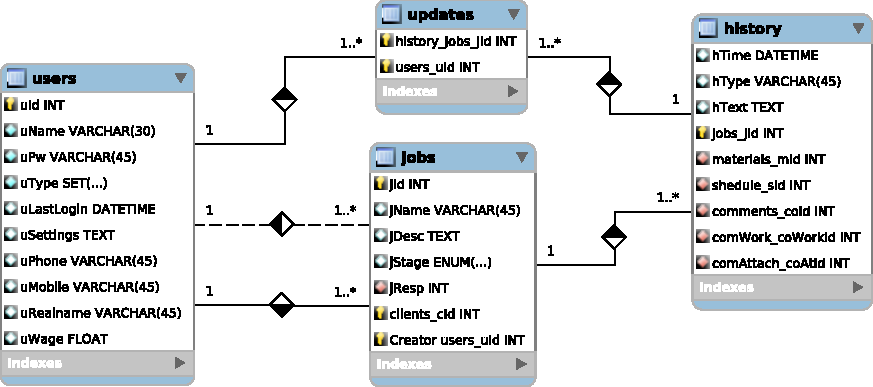
\includegraphics[scale=0.9]{./db_pdfs/history.pdf}
	\caption{Tabellen welche für die Benachrichtigungen (Updates) und Rückverfolgbarkeit zuständig sind.}
\end{figure}

\newpage
\section{Meilenstein 2}

\newpage
\section{Meilenstein 3}

\newpage
\section{Meilenstein 4}

\newpage
\section{Meilenstein 5}

\end{document}